% Source: https://tex.stackexchange.com/a/721901/6880

\documentclass{article}

\usepackage[margin=0pt]{geometry}%

\usepackage{tikz}
\usetikzlibrary{matrix}

\begin{document}

\centering
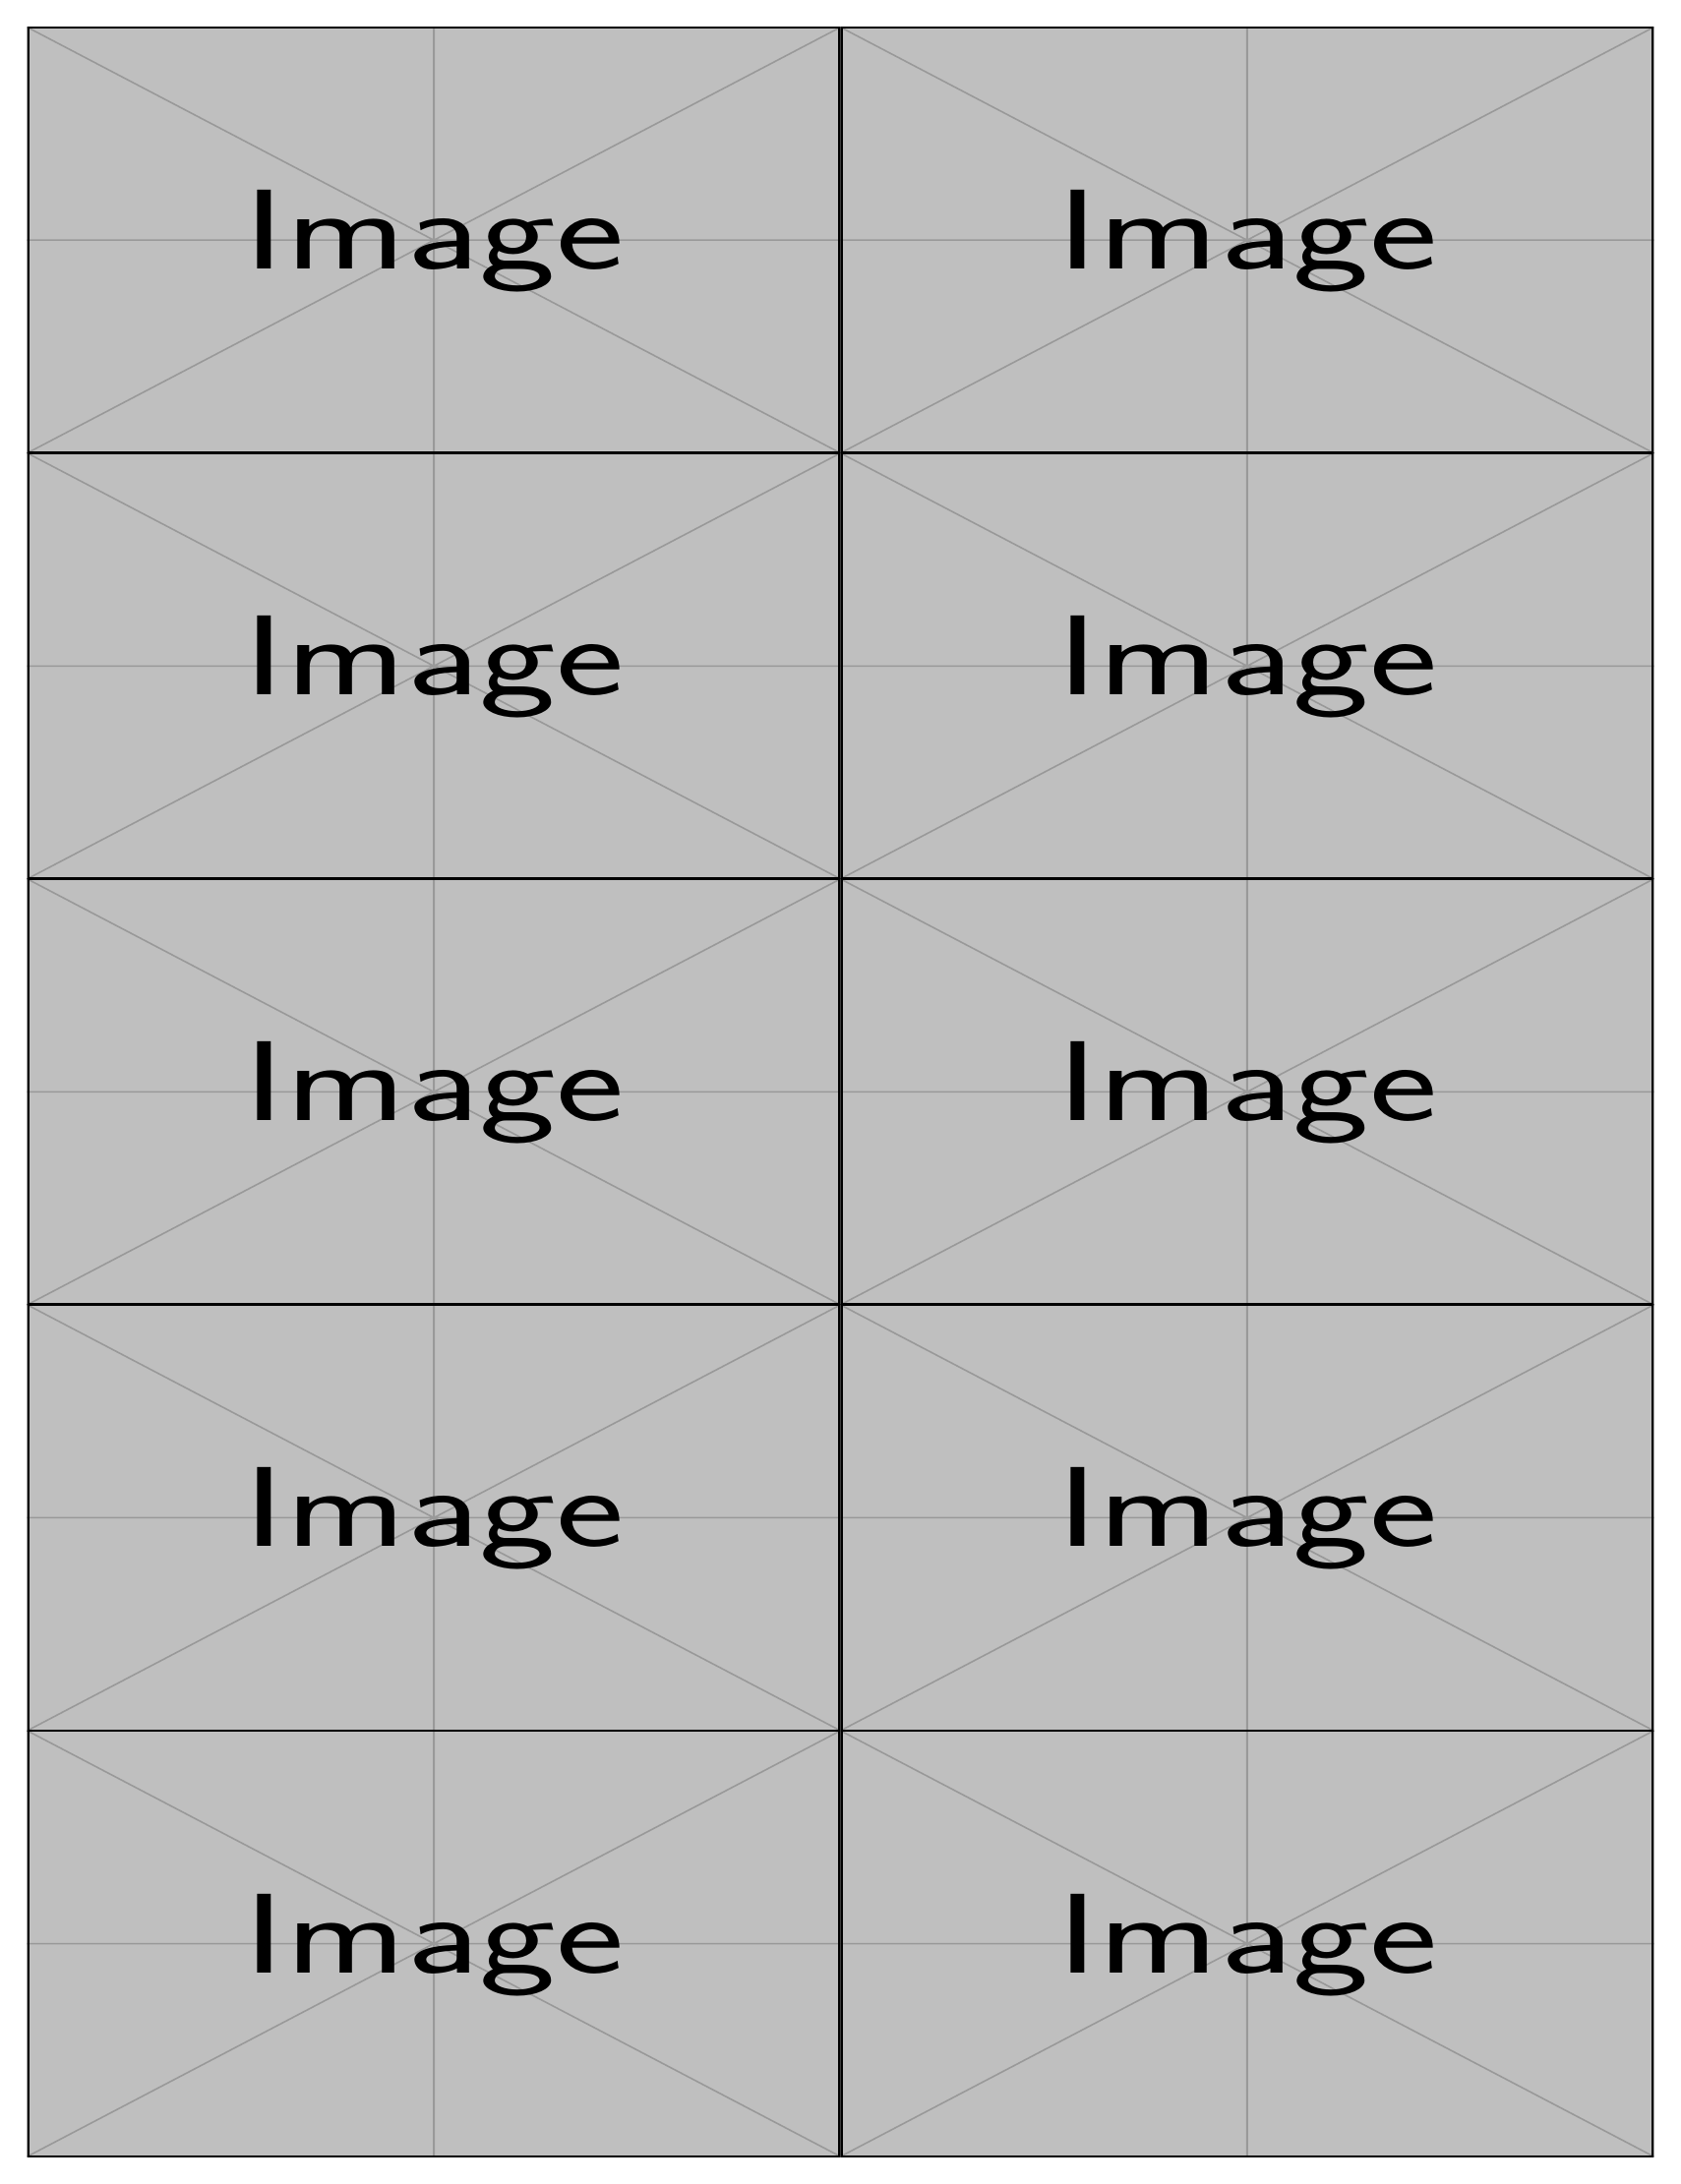
\begin{tikzpicture}
 \matrix(image)% <-- name added
    [matrix of nodes,nodes={scale=1,inner sep=0pt,outer sep=0pt},column sep=0pt,row sep=0pt,inner sep=0pt,outer sep=0pt]{
      \includegraphics[width=105mm,height=55mm]{example-image} 
    & \includegraphics[width=105mm,height=55mm]{example-image}
    \\ 
      \includegraphics[width=105mm,height=55mm]{example-image} 
    & \includegraphics[width=105mm,height=55mm]{example-image}
    \\ 
      \includegraphics[width=105mm,height=55mm]{example-image} 
    & \includegraphics[width=105mm,height=55mm]{example-image}
    \\ 
      \includegraphics[width=105mm,height=55mm]{example-image} 
    & \includegraphics[width=105mm,height=55mm]{example-image}
    \\ 
      \includegraphics[width=105mm,height=55mm]{example-image} 
    & \includegraphics[width=105mm,height=55mm]{example-image}
    \\ 
  };
% % Overlay text on each business card using the name of the matrix
%  \foreach \i in {1,...,5} {
%    \foreach \j in {1,2} {
%      \node[red,font=\bfseries\Huge] at (image-\i-\j) {John Doe};
%    }
%  }
 
\end{tikzpicture}

\end{document}
